\documentclass[border=10pt]{standalone}
\usepackage[svgnames]{xcolor}
\usepackage{amsmath}
\usepackage{pgfplots}
\pgfplotsset{compat=newest}
\usepackage[sfdefault]{FiraSans}
\usepackage{FiraMono}
\renewcommand*\familydefault{\sfdefault}
\begin{document}
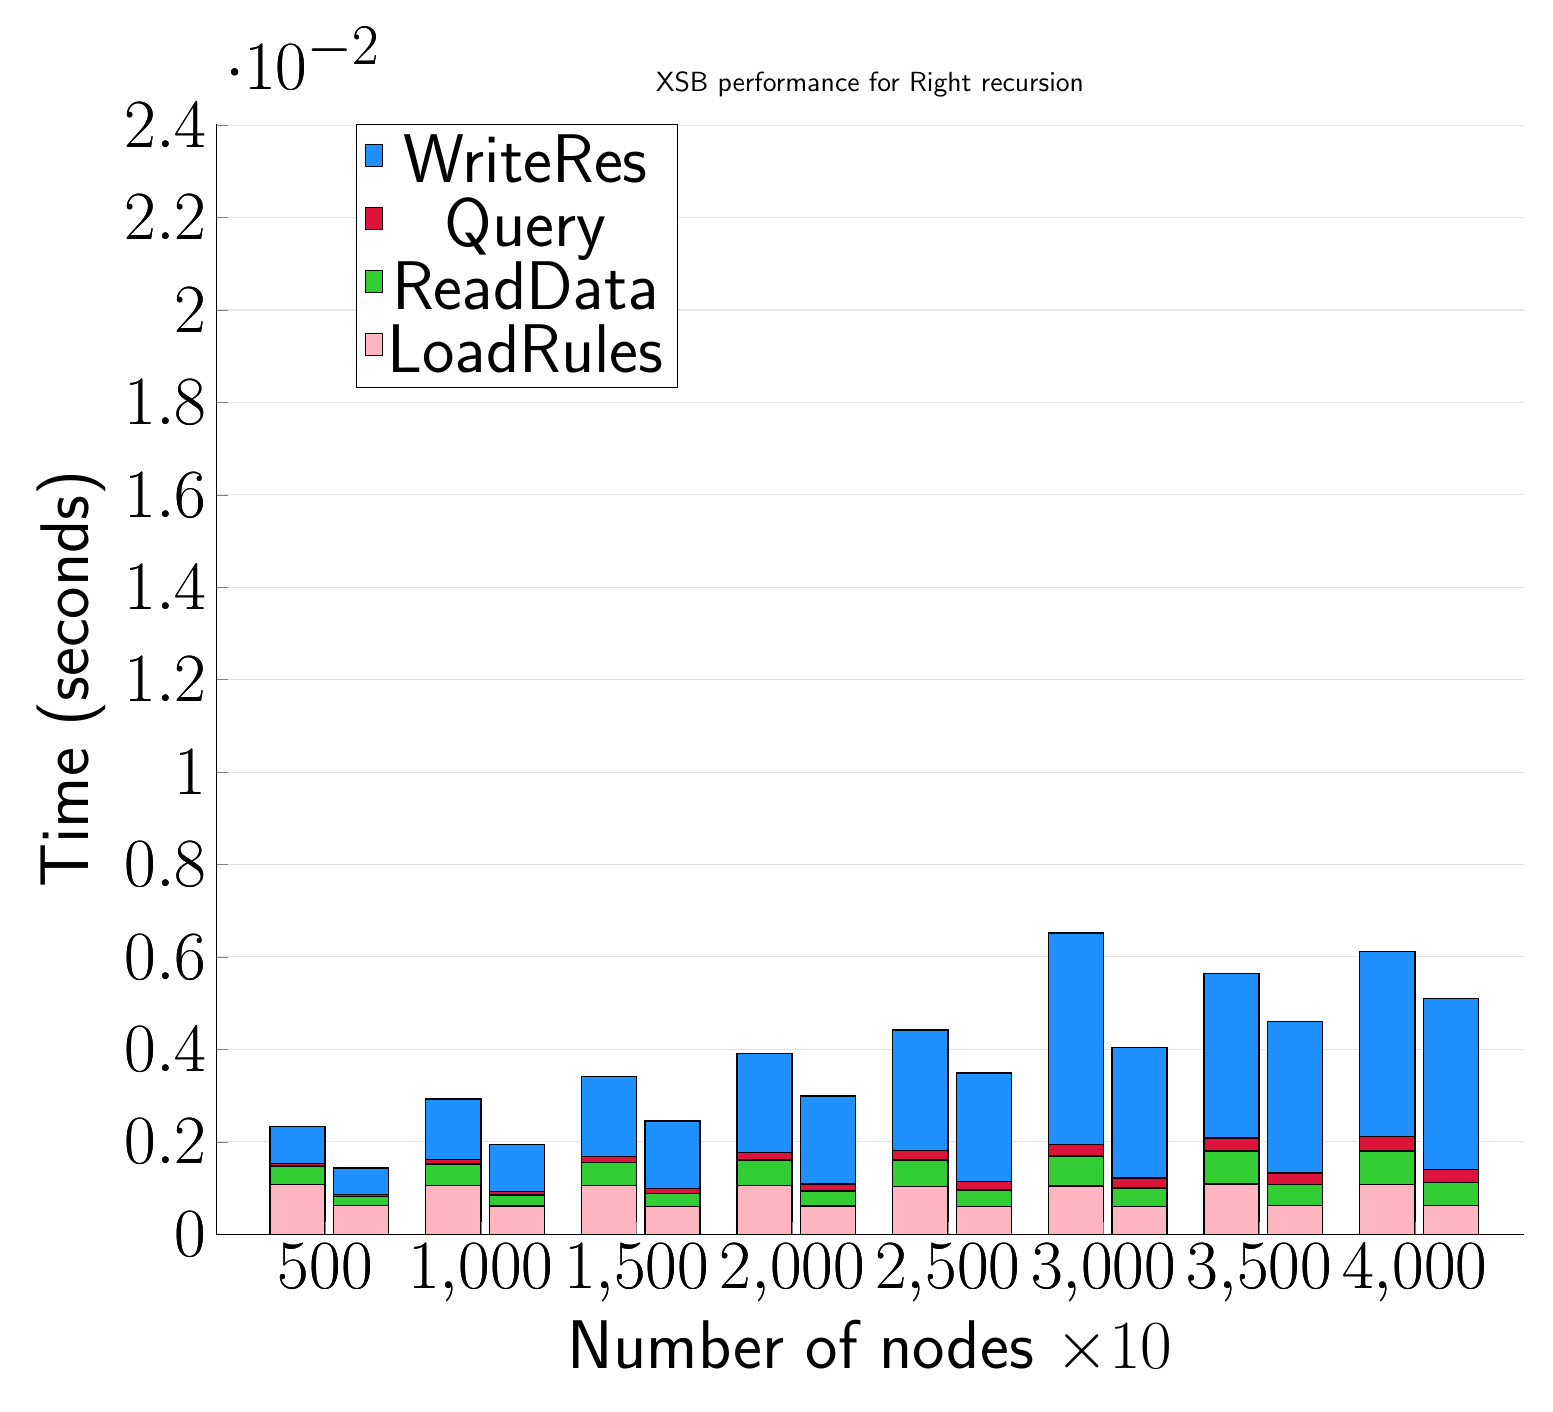
\begin{tikzpicture}
\begin{axis}[
   ybar stacked,
   title={XSB performance for Right recursion},
   bar shift=-10pt,
   width=1.5\textwidth,
   bar width=0.7cm,
   ymajorgrids, tick align=inside,
   major grid style={draw=gray!20},
   xtick=data,
   ymin=0, ymax=0.024034543037414553,
   axis x line*=bottom,
   axis y line*=left,
   enlarge x limits=0.1,
   legend style={
       at={(0.23, 1)},
       anchor=north,
       legend columns=1,
       font=\Huge,
   },
   ylabel={Time (seconds)},
   xlabel={Number of nodes $\times 10$},
   label style={font=\Huge},
   tick label style={font=\Huge},
]
\addlegendimage{fill=DodgerBlue, draw=black, line width=0.2pt}
\addlegendentry{WriteRes}
\addlegendimage{fill=Crimson, draw=black, line width=0.2pt}
\addlegendentry{Query}
\addlegendimage{fill=LimeGreen, draw=black, line width=0.2pt}
\addlegendentry{ReadData}
\addlegendimage{fill=LightPink, draw=black, line width=0.2pt}
\addlegendentry{LoadRules}
\addplot +[fill=LightPink, draw=black, line width=0.5pt] coordinates {
    (500, 0.0010718345642089838)
    (1000, 0.0010533809661865232)
    (1500, 0.0010553359985351553)
    (2000, 0.00105128288269043)
    (2500, 0.0010387659072875958)
    (3000, 0.0010473966598510739)
    (3500, 0.0010874032974243159)
    (4000, 0.0010708808898925778)
};
\addplot +[fill=LimeGreen, draw=black, line width=0.5pt] coordinates {
    (500, 0.00040116310119628904)
    (1000, 0.00046575069427490234)
    (1500, 0.0004957199096679687)
    (2000, 0.0005533456802368163)
    (2500, 0.0005673170089721679)
    (3000, 0.0006412267684936521)
    (3500, 0.0007095336914062498)
    (4000, 0.0007322549819946291)
};
\addplot +[fill=Crimson, draw=black, line width=0.5pt] coordinates {
    (500, 5.679130554199218e-05)
    (1000, 9.291172027587889e-05)
    (1500, 0.00013027191162109372)
    (2000, 0.0001699209213256835)
    (2500, 0.00020387172698974618)
    (3000, 0.00024616718292236334)
    (3500, 0.0002815008163452148)
    (4000, 0.00031578540802001926)
};
\addplot +[fill=DodgerBlue, draw=black, line width=0.5pt] coordinates {
    (500, 0.0007954359054565433)
    (1000, 0.0013116359710693363)
    (1500, 0.0017362356185913093)
    (2000, 0.0021394968032836916)
    (2500, 0.0026079177856445307)
    (3000, 0.004583549499511718)
    (3500, 0.003560376167297364)
    (4000, 0.0039952993392944345)
};
\end{axis}
\begin{axis}[
   ybar stacked,
   bar shift=13pt,
   width=1.5\textwidth,
   bar width=0.7cm,
   ymajorgrids, tick align=inside,
   major grid style={draw=none},
   xtick=data,
   ymin=0, ymax=0.024034543037414553,
   axis x line*=none,
   axis y line*=none,
   enlarge x limits=0.1,
   label style={font=\Huge},
   tick label style={font=\Huge},
]
\addplot +[fill=LightPink, draw=black, line width=0.5pt] coordinates {
    (500, 0.0006242000000000001)
    (1000, 0.0006126999999999998)
    (1500, 0.0006004000000000004)
    (2000, 0.0006112999999999998)
    (2500, 0.0006036000000000001)
    (3000, 0.0006012000000000002)
    (3500, 0.0006148999999999998)
    (4000, 0.0006182)
};
\addplot +[fill=LimeGreen, draw=black, line width=0.5pt] coordinates {
    (500, 0.0001862999999999999)
    (1000, 0.00023280000000000002)
    (1500, 0.0002747999999999997)
    (2000, 0.00032050000000000015)
    (2500, 0.0003552999999999999)
    (3000, 0.00040190000000000007)
    (3500, 0.0004582999999999995)
    (4000, 0.0004972)
};
\addplot +[fill=Crimson, draw=black, line width=0.5pt] coordinates {
    (500, 5.05000000000002e-05)
    (1000, 8.470000000000004e-05)
    (1500, 0.0001188)
    (2000, 0.0001522)
    (2500, 0.0001825999999999998)
    (3000, 0.00021719999999999907)
    (3500, 0.00025490000000000007)
    (4000, 0.0002850999999999997)
};
\addplot +[fill=DodgerBlue, draw=black, line width=0.5pt] coordinates {
    (500, 0.0005701999999999998)
    (1000, 0.0010142999999999997)
    (1500, 0.001454)
    (2000, 0.0019044)
    (2500, 0.0023501)
    (3000, 0.0028224000000000014)
    (3500, 0.0032812999999999996)
    (4000, 0.0037055000000000005)
};
\end{axis}
\end{tikzpicture}

\end{document}
